%%%%%%%%%%%%%%%%%%%%%%%%%%%%%%%%%%%%%%%%%%%%%%%%%%

\section{Domain Analysis of \hpl}
\label{sec:domainAnalysis}

Although tailored to managing variability in a specific SPL~\cite{ferreira:2010}, some users of \hp{} would appreciate more specific configurations of the tool. For instance, some users could be interested in managing variability only in requirements and use cases; others could be interested in managing variability only in source code; and yet other engineers could be interested in managing variabilities in requirements, use cases, and source code.  Accordingly, new extensions of \hp{} have been recently proposed. For instance, there exist variants of \hp{} supporting variability in business process models~\cite{Machado:2011:MVB:1960502.1960508} and \emph{Simulink} assets~\cite{simulink}.

These variants share the same configurability, flexibility, and extensibility issues explained in Section~\ref{sec:hephaestus}. To address these issues, we adopt a SPL perspective to \hp{} itself, thus leveraging the commonality in these variants and systematically managing the incurred variability. Since there are existing versions of \hp, we adopt the extractive strategy~\cite{kruegerPFE01}, bootstrapping the \hpl{} from such variants. Correspondingly, we analyzed the existing variants of \hp{} and manually identified the common and variable features, architectural and implementation elements. The remainder of this section explains the result of this strategy to identify commonality and variability among such elements. In Section~\ref{sec:domainDesign}, we present and explain how \hpl's domain design leverages this domain analysis and addresses configurability, flexibility, and extensibility; the details of implementation are presented in Section~\ref{sec:implementation}. Section~\ref{sec:process} details the reactive process needed to introduce support for managing variabilities in new assets.

%%%%%%%%%%%%%%%%%%%%%%%%%%%%%%%%%%%%%%%%%%%%%%%%%%

\begin{figure*}[bth]
\begin{center}
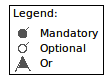
\includegraphics[width=.2\textwidth]{imagens/fm-hpl2.png}
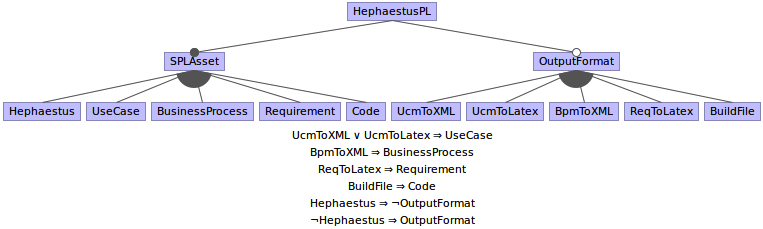
\includegraphics[width=\textwidth]{imagens/fm-hpl1.png}
\end{center}
\caption{\hpl's feature model. In this version, the features \textit{SPLAsset} and \textit{OutputFormat} define an \emph{or} relationship with their children}
\label{fig:hephaestus-fm-03}
\end{figure*}

%%%%%%%%%%%%%%%%%%%%%%%%%%%%%%%%%%%%%%%%%%%%%%%%%%

\subsection{\hpl's Feature Model} 
\label{feature-model-hpl}

In terms of the problem space, \hpl' feature model is represented in Figure~\ref{fig:hephaestus-fm-03}. As the diagram shows, the \emph{SPLAsset} feature is mandatory and the \emph{OutputFormat} feature; these features are parents of \emph{or-features} so that any combination of models and output formats is supported, e.g., a given instance might comprise business processes and use cases and export both assets as XML files. Managing variabilities in such a combination of features is essential in \hpl{} and has not been addressed elsewhere.

%%%%%%%%%%%%%%%%%%%%%%%%%%%%%%%%%%%%%%%%%%%%%%%%%%

\begin{figure*}[htb]
\begin{center}
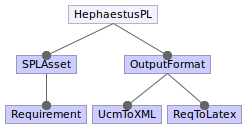
\includegraphics[scale=0.6]{imagens/confInvalid.png}
\end{center}
\caption{An invalid configuration of \hpl}
\label{fig:hephaestus-conf-invalid}
\end{figure*}

%%%%%%%%%%%%%%%%%%%%%%%%%%%%%%%%%%%%%%%%%%%%%%%%%%

In addition to the feature diagram, Figure~\ref{fig:hephaestus-fm-03} shows some cross tree constraints that must be satisfied for any valid feature configuration of \hpl.  To illustrate, Figure~\ref{fig:hephaestus-conf1a} and Figure~\ref{fig:hephaestus-conf1b} show two valid configurations of \hpl, whereas Figure~\ref{fig:hephaestus-conf-invalid} shows an invalid configuration of \hpl, in which the \emph{UcmToXML} feature is selected, but the \emph{UseCase} feature is not selected. In this case, the $UcmToXML \lor UcmToLatex \rightarrow Use Case$ constraint was violated, leading to an invalid feature configuration of \hpl.

Thus, in the problem space, a specific configuration of \hp{} is conceptually simple in that it is represented by a combination of a few \textit{or-features}. However, in the solution space, a specific configuration implies more complexity because it represents managing variability in a combination of artifacts (data types, functions of different kinds, and models) at different levels of granularity (i.e., course-grained and fine-grained), and the implementation of the features is somewhat scattered in \hp' source code.

%%%%%%%%%%%%%%%%%%%%%%%%%%%%%%%%%%%%%%%%%%%%%%%%%%

\subsection{Identification of Commonality} 
\label{commonality}

In the solution space, there exists significant amount of commonality among configurations. 
The domain analysis revealed \emph{commonality} for these abstractions across the variants of the evolution history:

\begin{itemize}

\item \emph{Feature Model Representation}: an algebraic data type represents the feature model of a product line.
  
\item \emph{Product Configuration Representation}: an algebraic data type represents a valid feature configuration.

\item \emph{Configuration Knowledge Representation} (CK Representation): an algebraic data type represents the product line's configuration knowledge.

\item \emph{Interpreter for Product Instantiation}: the \texttt{build} function performs the SPL instantiation by generating a product corresponding to a specific product line configuration.

\end{itemize}

%%%%%%%%%%%%%%%%%%%%%%%%%%%%%%%%%%%%%%%%%%%%%%%%%%

\subsection{Identification of Variability} 
\label{variability}

The domain analysis revealed \emph{variability} for these abstractions across the variants of the evolution history:

\begin{itemize}

\item \emph{Asset Representations}: algebraic data types represent the abstract syntax of different SPL assets (such as use cases, business processes, and code).

\item \emph{Asset Transformations}: functions manipulate such artifacts, solving variability of SPL assets. Some transformations basically select a specific asset from the product line, including it into the product during product derivation. Other transformations change the structure of an asset of the SPL in the final product.

\item \emph{Asset I/O}: parser/output functions for reading/writing artifacts convert the concrete syntax of an asset to/from the corresponding abstract syntax of \hpl{}, i.e., the asset abstract data types.

\item \emph{Asset Container}: the \texttt{SPLModel} and \texttt{InstanceModel} algebraic data types comprise the set of SPL assets and group it with the feature model or feature configuration, respectively, of a given \hpl{} instance.

\item \emph{Empty Instance}: an expression defines the initial representation of a product during the product derivation activity. It is an instance of the \texttt{InstanceModel} data type and serves as a baseline that is successively refined by the \texttt{build} function.

\item \emph{Configuration Knowledge Parser} (CK Parser): the \texttt{xml2Transformation} function parses the XML representation of transformations into actual transformations (functions) on instance models.

\end{itemize}

Domain analysis also substantiated that variability has a regular form that may be understood linguistically in terms of introduction of new abstractions (`modules') and extension of existing abstractions (data types and functions). For example, to introduce variability support for one new asset in \hp, one needs to implement the data types for representing the abstract syntax of these models, implement the transformations for solving variability, implement the parser and output functions for reading/writing these assets into/from \hp; one also needs to extend some data types and functions of \hp{}, as it was illustrated in Section~\ref{hp-evolution}.
